\documentclass[11pt,letterpaper,openany]{book}

% ============================================================================
% PACKAGES
% ============================================================================
\usepackage[utf8]{inputenc}
\usepackage[T1]{fontenc}
\usepackage{lmodern}
\usepackage[margin=1in]{geometry}
\usepackage{graphicx}
\usepackage{xcolor}
\usepackage{titlesec}
\usepackage{titletoc}
\usepackage{fancyhdr}
\usepackage{hyperref}
\usepackage{booktabs}
\usepackage{longtable}
\usepackage{tabularx}
\usepackage{array}
\usepackage{multirow}
\usepackage{enumitem}
\usepackage{parskip}
\usepackage{tocloft}
\usepackage{etoolbox}
\usepackage{pdfpages}
\usepackage{tcolorbox}
\usepackage{fontawesome5}
\usepackage{tikz}
\usepackage{pgfplots}
\pgfplotsset{compat=1.18}
\usepackage{amssymb}

% ============================================================================
% COLOR DEFINITIONS
% ============================================================================
\definecolor{gtgold}{RGB}{179,163,105}
\definecolor{gtnavy}{RGB}{0,48,87}
\definecolor{gtwhite}{RGB}{255,255,255}
\definecolor{cisoblue}{RGB}{31,78,121}
\definecolor{sectionblue}{RGB}{0,76,151}
\definecolor{lightgray}{RGB}{245,245,245}
\definecolor{accentgreen}{RGB}{0,128,0}
\definecolor{warnorange}{RGB}{230,126,34}

% ============================================================================
% HYPERREF CONFIGURATION
% ============================================================================
\hypersetup{
    colorlinks=true,
    linkcolor=cisoblue,
    filecolor=cisoblue,
    urlcolor=cisoblue,
    citecolor=cisoblue,
    pdftitle={OMS Cybersecurity CISO Career Guide},
    pdfauthor={Georgia Tech Professional Education},
    pdfsubject={Master of Science in Cybersecurity - CISO Track},
    pdfkeywords={Cybersecurity, CISO, Georgia Tech, OMS, Policy, Information Security}
}

% ============================================================================
% PAGE STYLE CONFIGURATION
% ============================================================================
\pagestyle{fancy}
\fancyhf{}
\fancyhead[LE,RO]{\thepage}
\fancyhead[RE]{\leftmark}
\fancyhead[LO]{\rightmark}
\renewcommand{\headrulewidth}{0.4pt}
\renewcommand{\footrulewidth}{0pt}

\fancypagestyle{plain}{
    \fancyhf{}
    \fancyfoot[C]{\thepage}
    \renewcommand{\headrulewidth}{0pt}
}

% ============================================================================
% TITLE FORMATTING
% ============================================================================
\titleformat{\chapter}[display]
    {\normalfont\huge\bfseries\color{gtnavy}}
    {\chaptertitlename\ \thechapter}{20pt}{\Huge}
\titlespacing*{\chapter}{0pt}{-20pt}{40pt}

\titleformat{\section}
    {\normalfont\Large\bfseries\color{sectionblue}}
    {\thesection}{1em}{}
\titleformat{\subsection}
    {\normalfont\large\bfseries\color{cisoblue}}
    {\thesubsection}{1em}{}
\titleformat{\subsubsection}
    {\normalfont\normalsize\bfseries}
    {\thesubsubsection}{1em}{}

% ============================================================================
% TABLE OF CONTENTS FORMATTING
% ============================================================================
\renewcommand{\cftchapfont}{\bfseries\color{gtnavy}}
\renewcommand{\cftsecfont}{\color{sectionblue}}
\renewcommand{\cftsubsecfont}{\color{cisoblue}}

% ============================================================================
% TCOLORBOX CONFIGURATIONS
% ============================================================================
\tcbuselibrary{skins,breakable}

\newtcolorbox{importantbox}{
    colback=lightgray,
    colframe=gtnavy,
    fonttitle=\bfseries,
    title=Key Information,
    breakable,
    enhanced
}

\newtcolorbox{notebox}{
    colback=blue!5,
    colframe=cisoblue,
    fonttitle=\bfseries,
    breakable,
    enhanced
}

\newtcolorbox{warningbox}{
    colback=orange!10,
    colframe=warnorange,
    fonttitle=\bfseries,
    title=Important Note,
    breakable,
    enhanced
}

\newtcolorbox{deliverablebox}[1][]{
    colback=green!5,
    colframe=accentgreen,
    fonttitle=\bfseries,
    title=#1,
    breakable,
    enhanced
}

% ============================================================================
% CUSTOM COMMANDS
% ============================================================================
\newcommand{\coursenum}[1]{\textbf{\textcolor{cisoblue}{#1}}}
\newcommand{\booktitle}[1]{\textit{#1}}
\newcommand{\term}[1]{\textbf{#1}}
\newcommand{\credits}[1]{(#1 credits)}

% ============================================================================
% DOCUMENT BEGIN
% ============================================================================
\begin{document}

% ============================================================================
% TITLE PAGE
% ============================================================================
\begin{titlepage}
    \centering
    \vspace*{1cm}
    
    \begin{tikzpicture}[remember picture,overlay]
        \fill[gtnavy] (current page.north west) rectangle ([yshift=-4cm]current page.north east);
    \end{tikzpicture}
    
    \vspace{1cm}
    
    {\color{gtgold}\rule{\linewidth}{2pt}}
    
    \vspace{1.5cm}
    
    {\Huge\bfseries\color{gtnavy} OMS Cybersecurity}\\[0.5cm]
    {\Huge\bfseries\color{gtnavy} CISO Career Guide}
    
    \vspace{1cm}
    
    {\color{gtgold}\rule{0.6\linewidth}{1pt}}
    
    \vspace{1.5cm}
    
    {\Large\color{cisoblue} A Comprehensive Academic and Professional\\[0.3cm]
    Development Framework for Aspiring\\[0.3cm]
    Chief Information Security Officers}
    
    \vspace{2cm}
    
    {\large\color{gtnavy}
    \textbf{Georgia Tech Professional Education}\\[0.3cm]
    Online Master of Science in Cybersecurity\\[0.3cm]
    Policy Specialization Track
    }
    
    \vfill
    
    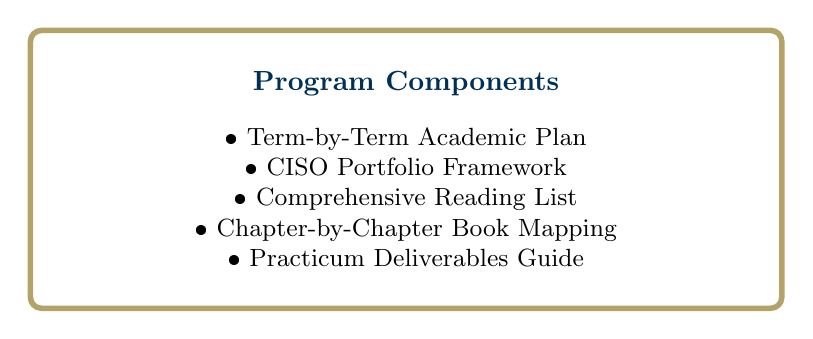
\begin{tikzpicture}
        \node[draw=gtgold,line width=2pt,rounded corners,inner sep=15pt] {
            \begin{minipage}{0.7\textwidth}
                \centering
                \textbf{\color{gtnavy}Program Components}\\[0.3cm]
                \small
                \textbullet~Term-by-Term Academic Plan\\
                \textbullet~CISO Portfolio Framework\\
                \textbullet~Comprehensive Reading List\\
                \textbullet~Chapter-by-Chapter Book Mapping\\
                \textbullet~Practicum Deliverables Guide
            \end{minipage}
        };
    \end{tikzpicture}
    
    \vspace{1cm}
    
    {\color{gtgold}\rule{\linewidth}{2pt}}
    
    \vspace{0.5cm}
    
    {\small\color{gray} Document Version 1.0 | January 2026}
    
\end{titlepage}

% ============================================================================
% COPYRIGHT/DISCLAIMER PAGE
% ============================================================================
\thispagestyle{empty}
\vspace*{\fill}
\begin{center}
    \textit{This document is intended as a comprehensive planning guide for students pursuing the Online Master of Science in Cybersecurity at Georgia Institute of Technology with career aspirations toward Chief Information Security Officer (CISO) roles.}
    
    \vspace{1cm}
    
    \textit{Course offerings, prerequisites, and program requirements are subject to change. Students should verify all information with official Georgia Tech sources before making academic decisions.}
    
    \vspace{2cm}
    
    \textbf{Official Resources:}\\[0.5cm]
    \url{https://pe.gatech.edu/degrees/cybersecurity}\\
    \url{https://pe.gatech.edu/degrees/cybersecurity/curriculum}
\end{center}
\vspace*{\fill}
\newpage

% ============================================================================
% TABLE OF CONTENTS
% ============================================================================
\tableofcontents
\newpage

% ============================================================================
% PART I: EXECUTIVE OVERVIEW
% ============================================================================
\part{Program Overview and Strategic Framework}

\chapter{Introduction to the CISO Career Path}

\section{Executive Summary}

This document presents a comprehensive, CISO-optimized approach to the Georgia Tech Online Master of Science in Cybersecurity (OMS Cybersecurity) program. The framework is designed to provide aspiring Chief Information Security Officers with both the policy and governance expertise required for executive leadership and the technical depth necessary to maintain credibility with engineering teams, auditors, and boards.

The strategy recommends declaring the \textbf{Policy specialization} as the primary track, which formalizes governance, regulation, privacy, geopolitics, and executive-level security management, while deliberately supplementing the curriculum with Information Security technical courses beyond the minimum requirements.

\section{Why the Policy Track for CISO Aspirants}

The Policy track represents the cleanest pathway for future CISOs because:

\begin{itemize}[leftmargin=*]
    \item \textbf{Executive Communication:} Policy courses emphasize board-level communication, regulatory compliance, and strategic risk management
    \item \textbf{Governance Foundations:} Direct exposure to IT governance frameworks, decision rights, and enterprise security management
    \item \textbf{Regulatory Depth:} Comprehensive coverage of privacy law, ICT policy, and international security frameworks
    \item \textbf{Strategic Perspective:} Geopolitical and economic dimensions of cybersecurity that inform enterprise strategy
\end{itemize}

The technical credibility gap is addressed through strategic selection of Information Security track courses as electives and additional coursework beyond degree requirements.

\section{Program Structure Overview}

The OMS Cybersecurity program requires 32 credit hours distributed as follows:

\begin{table}[h]
\centering
\begin{tabular}{lcc}
\toprule
\textbf{Component} & \textbf{Credit Hours} & \textbf{Courses} \\
\midrule
Interdisciplinary Core & 6 & 2 \\
Flexible Core & 3 & 1 \\
Track Coursework & 18 & 6 \\
Practicum & 5 & 1 \\
\midrule
\textbf{Total} & \textbf{32} & \textbf{10} \\
\bottomrule
\end{tabular}
\caption{OMS Cybersecurity Degree Requirements}
\end{table}

\begin{importantbox}
\textbf{Practicum Eligibility Requirements:}
\begin{itemize}[leftmargin=*,noitemsep]
    \item Minimum of 8 completed courses (with grade C or higher)
    \item Must include CS 6035 and PUBP 6725
    \item Prerequisites must be completed \textit{before} (not concurrent with) practicum enrollment
\end{itemize}
\end{importantbox}

% ============================================================================
% CHAPTER: DEGREE PLAN
% ============================================================================
\chapter{Complete Degree Plan}

\section{Interdisciplinary Core (6 Credit Hours)}

The interdisciplinary core establishes the foundational bridge between technical security and policy perspectives. Both courses are required for all students regardless of track.

\subsection{CS 6035 --- Introduction to Information Security}

\begin{notebox}
\textbf{Course Overview:} This course provides a broad introduction to the field of information security, covering topics including software security, operating system security, network security, applied cryptography, human factors, and policy.

\textbf{Strategic Value:} Serves as the prerequisite for most advanced security courses and establishes common technical vocabulary for cross-functional communication.
\end{notebox}

\subsection{PUBP 6725 --- Information Security Policies and Strategies}

\begin{notebox}
\textbf{Course Overview:} Examines the policy dimensions of information security, including risk management frameworks, compliance requirements, governance structures, and strategic planning for security programs.

\textbf{Strategic Value:} Directly applicable to CISO responsibilities including security program design, policy development, and stakeholder communication.
\end{notebox}

\section{Flexible Core (3 Credit Hours)}

The flexible core requires one course from a different track than the declared specialization. For Policy track students, this provides an opportunity to establish technical credentials.

\subsection{CS 6262 --- Network Security (Recommended)}

\begin{notebox}
\textbf{Course Overview:} Covers network security fundamentals including firewalls, intrusion detection systems, VPNs, secure protocols, and network-based attacks and defenses.

\textbf{Strategic Value:} Essential for CISO credibility when discussing infrastructure security, network architecture decisions, and SOC operations.
\end{notebox}

\section{Policy Track Required Courses (12 Credit Hours)}

Select four courses from the Policy track required list. The following selections maximize CISO relevance across privacy, enterprise governance, geopolitical risk, and policy mechanisms.

\subsection{PUBP 8833 --- Enterprise Cybersecurity}

\begin{notebox}
\textbf{Course Overview:} Focuses on managing cybersecurity at the enterprise level, including security operating models, governance frameworks, program development, and board-level reporting.

\textbf{Strategic Value:} Directly maps to core CISO responsibilities and practicum deliverables. Essential for understanding how to structure and lead a security organization.
\end{notebox}

\subsection{MGT 6727 --- Privacy for Professionals}

\begin{notebox}
\textbf{Course Overview:} Comprehensive examination of privacy law, regulations, and governance including GDPR, CCPA, HIPAA, and sector-specific requirements.

\textbf{Strategic Value:} Privacy is a board-level concern and increasingly intertwined with security. Essential for regulatory compliance and data governance leadership.
\end{notebox}

\subsection{PUBP 6502 --- Information and Communications Technology Policy}

\begin{notebox}
\textbf{Course Overview:} Examines the policy landscape affecting information and communications technology, including regulatory frameworks, standards development, and policy-making processes.

\textbf{Strategic Value:} Understanding policy levers and regulatory dynamics is essential for anticipating compliance requirements and engaging with regulators.
\end{notebox}

\subsection{PUBP 8823 --- Geopolitics of Cybersecurity}

\begin{notebox}
\textbf{Course Overview:} Analyzes the intersection of cybersecurity and international relations, including state-sponsored threats, cyber warfare, international law, and diplomatic dimensions of security.

\textbf{Strategic Value:} Essential for threat intelligence context, understanding advanced persistent threats, and strategic risk assessment in global organizations.
\end{notebox}

\section{Policy Track Elective Courses (6 Credit Hours)}

Select two additional courses from the Policy track elective list. The following selections strengthen executive-level threat framing and security strategy.

\subsection{INTA 6103 --- International Security}

\begin{notebox}
\textbf{Course Overview:} Broad examination of international security concepts, theories, and contemporary challenges including terrorism, proliferation, and regional conflicts.

\textbf{Strategic Value:} Provides framework for understanding the broader security environment in which cyber threats operate.
\end{notebox}

\subsection{INTA 6450 --- Big Data and Security}

\begin{notebox}
\textbf{Course Overview:} Explores the intersection of big data analytics and security, including intelligence applications, privacy implications, and data-driven security operations.

\textbf{Strategic Value:} Relevant to security analytics, SIEM/SOAR strategy, and data governance in modern security programs.
\end{notebox}

\section{Practicum (5 Credit Hours)}

\subsection{PUBP 6266 --- Policy Practicum}

\begin{deliverablebox}[Practicum Topic Recommendation]
\textbf{CISO-Credible Practicum Project:}

Design and justify an enterprise cybersecurity program for a specific organization (real or sponsored), including:
\begin{itemize}[leftmargin=*,noitemsep]
    \item Risk register methodology and governance cadence
    \item Control framework mapping (NIST CSF/800-53, ISO 27001)
    \item Metrics and KRI/KPI catalog with dashboard specifications
    \item IR governance and playbook framework
    \item Board reporting pack and executive communication materials
    \item Security operating model with RACI and staffing plan
    \item 12--18 month strategic roadmap with milestones
\end{itemize}
\end{deliverablebox}

The practicum can typically be completed with an employer or external sponsor, providing an opportunity to create real-world artifacts that demonstrate CISO-level competency.

% ============================================================================
% CHAPTER: TECHNICAL ADD-ON SEQUENCE
% ============================================================================
\chapter{Technical Credibility Enhancement}

\section{Rationale for Additional Technical Coursework}

While the Policy track provides essential governance and strategic foundations, CISOs must maintain technical authority that stands up with engineers, auditors, and boards. The following courses, taken beyond degree requirements, establish deep technical credibility.

\section{Information Security Technical Backbone}

These courses form the core technical spine that every security leader should understand.

\subsection{CS 6260 --- Applied Cryptography}

\begin{notebox}
\textbf{Prerequisites:} CS 6035

\textbf{Course Overview:} Covers cryptographic primitives, protocols, and their applications including symmetric and asymmetric encryption, hash functions, digital signatures, and key management.

\textbf{Strategic Value:} Essential for understanding encryption requirements, PKI infrastructure, and cryptographic controls in compliance frameworks.
\end{notebox}

\subsection{CS 6238 --- Secure Computer Systems}

\begin{notebox}
\textbf{Prerequisites:} CS 6035 (OS background recommended)

\textbf{Course Overview:} Examines security mechanisms in operating systems and distributed systems including access control, isolation, secure boot, and trusted computing.

\textbf{Strategic Value:} Foundation for understanding endpoint security, zero trust architecture, and platform security decisions.
\end{notebox}

\subsection{CS 6264 or CS 6265 --- Information Security Laboratory}

\begin{notebox}
\textbf{Prerequisites:} CS 6238 and CS 6262

\textbf{Course Overview:} Hands-on laboratory experience in offensive and defensive security techniques including vulnerability analysis, exploitation, and defense mechanisms.

\textbf{Strategic Value:} Provides hands-on credibility essential for leading penetration testing programs and understanding real-world attack techniques.
\end{notebox}

\section{Security Operations and Incident Leadership}

\subsection{Security Incident Response}

\begin{notebox}
\textbf{Course Overview:} Covers incident detection, containment, eradication, recovery, and lessons learned processes. Includes crisis communication and regulatory notification requirements.

\textbf{Strategic Value:} Direct preparation for leading IR teams and managing security crises at the executive level.
\end{notebox}

\section{Platform Fundamentals}

Understanding modern infrastructure is essential for governing cloud risk and architectural decisions.

\subsection{CS 6250 --- Computer Networks}

\begin{notebox}
\textbf{Course Overview:} Comprehensive coverage of network architecture, protocols, and performance including TCP/IP, routing, congestion control, and network design.

\textbf{Strategic Value:} Essential foundation for network security decisions and understanding SOC operations.
\end{notebox}

\subsection{CS 6210 --- Advanced Operating Systems}

\begin{notebox}
\textbf{Course Overview:} Deep dive into operating system design including process management, memory management, file systems, and distributed systems concepts.

\textbf{Strategic Value:} Supports understanding of secure system design, containerization, and platform security.
\end{notebox}

\subsection{CS 6300 --- Software Development Process}

\begin{notebox}
\textbf{Course Overview:} Software engineering principles including development methodologies, testing, quality assurance, and project management.

\textbf{Strategic Value:} Essential for leading application security programs and integrating security into SDLC.
\end{notebox}

\subsection{CS 6400 --- Database System Concepts and Design}

\begin{notebox}
\textbf{Course Overview:} Database design, implementation, and management including relational models, SQL, transactions, and performance optimization.

\textbf{Strategic Value:} Foundation for data security governance and understanding database security controls.
\end{notebox}

\section{Threats, Malware, and Defense Research}

\subsection{CS 6747 --- Advanced Topics in Malware Analysis}

\begin{notebox}
\textbf{Course Overview:} Advanced techniques for analyzing sophisticated malware including anti-analysis techniques, advanced persistent threats, and automated analysis.

\textbf{Strategic Value:} Informs detection engineering strategy and threat intelligence program development.
\end{notebox}

\subsection{CS 8813 --- Malware Analysis and Defense}

\begin{notebox}
\textbf{Course Overview:} Comprehensive coverage of malware analysis techniques and defensive countermeasures.

\textbf{Strategic Value:} Essential for understanding threat landscape and leading endpoint security programs.
\end{notebox}

\section{Critical Infrastructure and Hardware Security (Optional)}

For CISOs in regulated or industrial domains (energy, manufacturing, IoT), additional hardware-oriented security courses provide essential domain expertise.

\subsection{ECE 6770 --- Introduction to Cyber-Physical Systems Security}

\begin{notebox}
\textbf{Course Overview:} Security challenges unique to cyber-physical systems including SCADA, industrial control systems, and IoT devices.

\textbf{Strategic Value:} Essential for CISOs in OT environments or organizations with significant IoT exposure.
\end{notebox}

\subsection{ECE 8843 --- Side-Channels and Their Role in Cybersecurity}

\begin{notebox}
\textbf{Course Overview:} Side-channel attacks and defenses including timing attacks, power analysis, and electromagnetic emanations.

\textbf{Strategic Value:} Important for hardware security governance and supply chain security programs.
\end{notebox}

\subsection{ECE 8873 --- Advanced Hardware Oriented Security and Trust}

\begin{notebox}
\textbf{Course Overview:} Hardware security primitives, trusted platform modules, and hardware root of trust implementations.

\textbf{Strategic Value:} Foundation for hardware security requirements and supply chain integrity programs.
\end{notebox}

% ============================================================================
% PART II: TERM-BY-TERM PLAN
% ============================================================================
\part{Academic Execution Plan}

\chapter{Term-by-Term Schedule}

This chapter presents a prerequisite-aware, term-by-term academic plan that completes the OMS Cybersecurity degree while building dual credibility across Policy/GRC and technical Information Security domains.

\section{Planning Assumptions}

\begin{itemize}[leftmargin=*]
    \item \textbf{Declared Specialization:} Policy
    \item \textbf{Course Load:} 2 courses per regular term, 1 course in summer
    \item \textbf{Target Completion:} 3 years for degree requirements
    \item \textbf{Extended Plan:} Year 4+ for additional technical credibility courses
\end{itemize}

\section{Year 1 --- Build Foundations}

\subsection{Fall Semester (2 Courses)}

\begin{table}[h]
\centering
\begin{tabularx}{\textwidth}{lXc}
\toprule
\textbf{Course} & \textbf{Strategic Purpose} & \textbf{Credits} \\
\midrule
\coursenum{CS 6035} & Introduction to Information Security --- Core foundation, unlocks multiple security courses & 3 \\
\coursenum{CS 6250} & Computer Networks --- Precursor for Network Security, builds architecture fluency & 3 \\
\bottomrule
\end{tabularx}
\end{table}

\subsection{Spring Semester (2 Courses)}

\begin{table}[h]
\centering
\begin{tabularx}{\textwidth}{lXc}
\toprule
\textbf{Course} & \textbf{Strategic Purpose} & \textbf{Credits} \\
\midrule
\coursenum{PUBP 6725} & Information Security Policies and Strategies --- Core policy foundation & 3 \\
\coursenum{CS 6262} & Network Security --- Technical depth, benefits from Networks foundation & 3 \\
\bottomrule
\end{tabularx}
\end{table}

\subsection{Summer Semester (1 Course)}

\begin{table}[h]
\centering
\begin{tabularx}{\textwidth}{lXc}
\toprule
\textbf{Course} & \textbf{Strategic Purpose} & \textbf{Credits} \\
\midrule
\coursenum{CS 6210} & Advanced Operating Systems --- Supports Secure Computer Systems prerequisites & 3 \\
\bottomrule
\end{tabularx}
\end{table}

\begin{importantbox}
\textbf{Year 1 Summary:} 5 courses completed (15 credits)

At the end of Year 1, you have established both policy (PUBP 6725) and technical (CS 6035, CS 6262, CS 6250, CS 6210) foundations.
\end{importantbox}

\section{Year 2 --- Deepen Leadership and Reach Practicum Eligibility}

\subsection{Fall Semester (2 Courses)}

\begin{table}[h]
\centering
\begin{tabularx}{\textwidth}{lXc}
\toprule
\textbf{Course} & \textbf{Strategic Purpose} & \textbf{Credits} \\
\midrule
\coursenum{CS 6238} & Secure Computer Systems --- Prereq: CS 6035, benefits from OS background & 3 \\
\coursenum{PUBP 8833} & Enterprise Cybersecurity --- CISO governance and program lens & 3 \\
\bottomrule
\end{tabularx}
\end{table}

\subsection{Spring Semester (2 Courses)}

\begin{table}[h]
\centering
\begin{tabularx}{\textwidth}{lXc}
\toprule
\textbf{Course} & \textbf{Strategic Purpose} & \textbf{Credits} \\
\midrule
\coursenum{MGT 6727} & Privacy for Professionals --- Privacy governance, board/regulatory domain & 3 \\
\coursenum{PUBP 6502} & Information \& Communications Technology Policy --- Policy lever comprehension & 3 \\
\bottomrule
\end{tabularx}
\end{table}

\begin{importantbox}
\textbf{Practicum Eligibility Checkpoint:}

At this point you have \textbf{9 completed courses}, including CS 6035 and PUBP 6725. You meet the minimum 8-course requirement for practicum eligibility.
\end{importantbox}

\subsection{Summer Semester (Options)}

\textbf{Option A (Recommended):} Begin practicum application and project definition work. Practicum term availability varies; consult with program advisors.

\textbf{Option B:} Take \coursenum{PUBP 8823} (Geopolitics of Cybersecurity) if you prefer to start practicum in Fall.

\section{Year 3 --- Practicum and Technical Authority}

\subsection{Fall Semester (Practicum)}

\begin{table}[h]
\centering
\begin{tabularx}{\textwidth}{lXc}
\toprule
\textbf{Course} & \textbf{Strategic Purpose} & \textbf{Credits} \\
\midrule
\coursenum{CS/ECE/PUBP 6727} & Cybersecurity Practicum --- Capstone project with employer/sponsor & 5 \\
\bottomrule
\end{tabularx}
\end{table}

\begin{warningbox}
The practicum requires a permit and completed prerequisites. All prerequisite courses must be completed \textit{before} practicum enrollment, not taken concurrently.
\end{warningbox}

\subsection{Spring Semester (2 Courses --- Technical Authority)}

\begin{table}[h]
\centering
\begin{tabularx}{\textwidth}{lXc}
\toprule
\textbf{Course} & \textbf{Strategic Purpose} & \textbf{Credits} \\
\midrule
\coursenum{CS 6260} & Applied Cryptography --- Prereq: CS 6035, cryptographic foundations & 3 \\
\coursenum{CS 6265} & Information Security Lab --- Prereqs: CS 6238 + CS 6262, hands-on credibility & 3 \\
\bottomrule
\end{tabularx}
\end{table}

\subsection{Summer Semester (1 Course)}

\begin{table}[h]
\centering
\begin{tabularx}{\textwidth}{lXc}
\toprule
\textbf{Course} & \textbf{Strategic Purpose} & \textbf{Credits} \\
\midrule
\coursenum{INTA 6103} or \coursenum{INTA 6450} & International Security or Big Data and Security --- Choose based on industry target & 3 \\
\bottomrule
\end{tabularx}
\end{table}

\begin{importantbox}
\textbf{Degree Completion:} At the end of Year 3, you have completed all 32 credit hours required for the OMS Cybersecurity degree.
\end{importantbox}

\section{Year 4+ --- CISO Technical and Operational Mastery}

These courses are not required for the degree but materially increase CISO credibility with engineering, SOC, and audit teams.

\subsection{Recommended Additional Courses}

\begin{table}[h]
\centering
\begin{tabularx}{\textwidth}{llX}
\toprule
\textbf{Term} & \textbf{Course} & \textbf{Purpose} \\
\midrule
Fall & CS 6300 & Software Development Process --- AppSec program leadership \\
Fall & CS 6400 & Databases --- Data security governance \\
Spring & CS 6255 & Network Management --- Monitoring/operations posture \\
Spring & CS 6365 & Enterprise Computing --- Enterprise architecture patterns \\
Summer & CS 8813/6747 & Malware Analysis --- Threat understanding, detection engineering \\
\bottomrule
\end{tabularx}
\end{table}

\section{Visual Timeline}

\begin{figure}[h]
\centering
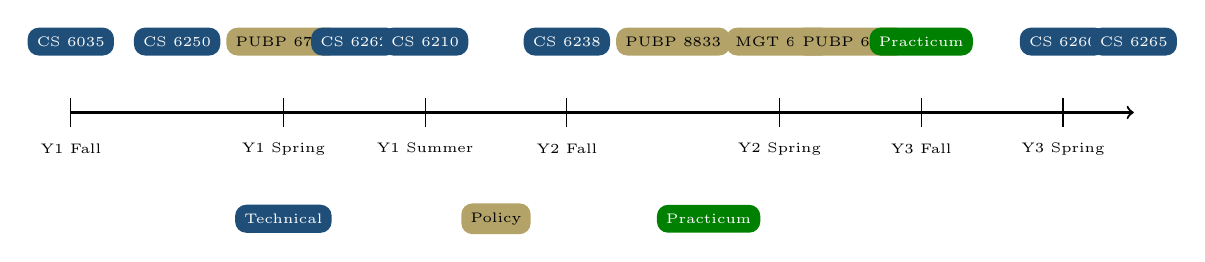
\begin{tikzpicture}[scale=0.9]
    % Timeline
    \draw[thick,->] (0,0) -- (15,0);
    
    % Year markers
    \foreach \x/\year in {0/Y1 Fall, 3/Y1 Spring, 5/Y1 Summer, 7/Y2 Fall, 10/Y2 Spring, 12/Y3 Fall, 14/Y3 Spring} {
        \draw (\x,-0.2) -- (\x,0.2);
        \node[below] at (\x,-0.3) {\tiny\year};
    }
    
    % Course nodes
    \node[fill=cisoblue,text=white,rounded corners,font=\tiny] at (0,1) {CS 6035};
    \node[fill=cisoblue,text=white,rounded corners,font=\tiny] at (1.5,1) {CS 6250};
    \node[fill=gtgold,text=black,rounded corners,font=\tiny] at (3,1) {PUBP 6725};
    \node[fill=cisoblue,text=white,rounded corners,font=\tiny] at (4,1) {CS 6262};
    \node[fill=cisoblue,text=white,rounded corners,font=\tiny] at (5,1) {CS 6210};
    \node[fill=cisoblue,text=white,rounded corners,font=\tiny] at (7,1) {CS 6238};
    \node[fill=gtgold,text=black,rounded corners,font=\tiny] at (8.5,1) {PUBP 8833};
    \node[fill=gtgold,text=black,rounded corners,font=\tiny] at (10,1) {MGT 6727};
    \node[fill=gtgold,text=black,rounded corners,font=\tiny] at (11,1) {PUBP 6502};
    \node[fill=accentgreen,text=white,rounded corners,font=\tiny] at (12,1) {Practicum};
    \node[fill=cisoblue,text=white,rounded corners,font=\tiny] at (14,1) {CS 6260};
    \node[fill=cisoblue,text=white,rounded corners,font=\tiny] at (15,1) {CS 6265};
    
    % Legend
    \node[fill=cisoblue,text=white,rounded corners,font=\tiny] at (3,-1.5) {Technical};
    \node[fill=gtgold,text=black,rounded corners,font=\tiny] at (6,-1.5) {Policy};
    \node[fill=accentgreen,text=white,rounded corners,font=\tiny] at (9,-1.5) {Practicum};
\end{tikzpicture}
\caption{Course Sequencing Timeline}
\end{figure}

% ============================================================================
% PART III: CISO PORTFOLIO
% ============================================================================
\part{CISO Portfolio Framework}

\chapter{Practicum Deliverables as CISO Portfolio}

The practicum is your opportunity to produce a CISO-grade portfolio: artifacts that demonstrate what a real security leader would bring to an executive team and board. This chapter maps the portfolio structure to specific deliverables.

\section{Portfolio Structure Overview}

Create a comprehensive CISO Portfolio with six integrated sections. Each section demonstrates a core CISO competency and produces artifacts suitable for professional use.

\begin{table}[h]
\centering
\begin{tabularx}{\textwidth}{lX}
\toprule
\textbf{Section} & \textbf{Demonstrates} \\
\midrule
A. Board Deck & Executive communication and risk framing \\
B. Metrics System & Measurement of security outcomes and operations \\
C. Risk Program & Enterprise security risk management \\
D. Security Org Design & Ability to build and lead the security function \\
E. IR Playbooks & Crisis leadership and institutionalized response \\
F. Roadmap & Strategic execution across people/process/technology \\
\bottomrule
\end{tabularx}
\end{table}

\section{Section A: Board Deck (Executive Communications Pack)}

\subsection{Purpose}
Demonstrate ability to brief leadership with clarity, risk framing, and decision asks.

\subsection{Deliverables}

\begin{deliverablebox}[Board Deck Contents]
\begin{itemize}[leftmargin=*,noitemsep]
    \item 10--15 slide board presentation
    \item 1--2 page executive read-ahead document
    \item Top risks (5--10) with trend lines and material risk narrative
    \item Current posture vs. target posture (capabilities model)
    \item Major initiatives: scope, timeline, cost, expected risk reduction
    \item Decision requests: policy approvals, funding, staffing, risk acceptance
\end{itemize}
\end{deliverablebox}

\subsection{Quality Criteria}
\begin{itemize}[leftmargin=*]
    \item Meeting-ready presentation quality
    \item Minimal jargon, accessible to non-technical executives
    \item Clearly stated decision points and recommendations
    \item Visual risk trends and maturity progression
\end{itemize}

\section{Section B: Metrics and Reporting System}

\subsection{Purpose}
Show ability to measure security outcomes and operational performance with rigor.

\subsection{Deliverables}

\begin{deliverablebox}[Metrics Framework Contents]
\begin{itemize}[leftmargin=*,noitemsep]
    \item \textbf{Metrics Catalog:} Definition, formula, data source, owner, cadence for each metric
    \item \textbf{Key Risk Indicators (KRIs):}
    \begin{itemize}[noitemsep]
        \item Control failure rates
        \item Critical vulnerability aging
        \item Phishing susceptibility rates
        \item Third-party risk scores
    \end{itemize}
    \item \textbf{Key Performance Indicators (KPIs):}
    \begin{itemize}[noitemsep]
        \item Patch SLA attainment
        \item Mean Time to Detect/Respond (MTTD/MTTR)
        \item Incident volume by severity
        \item Coverage metrics (EDR, logging, etc.)
    \end{itemize}
    \item \textbf{North-star Metrics:} Risk reduction, business enablement indicators
    \item \textbf{Dashboard Wireframes:} Visual specifications for reporting
\end{itemize}
\end{deliverablebox}

\subsection{Integration Requirements}
\begin{itemize}[leftmargin=*]
    \item Metrics must tie to roadmap initiatives
    \item KRIs must connect to risk register entries
    \item Dashboard design must support board-level and operational views
\end{itemize}

\section{Section C: Risk Program}

\subsection{Purpose}
Prove ability to run enterprise security risk management.

\subsection{Deliverables}

\begin{deliverablebox}[Risk Management Playbook]
\begin{itemize}[leftmargin=*,noitemsep]
    \item \textbf{Risk Methodology:}
    \begin{itemize}[noitemsep]
        \item Likelihood/impact scales with definitions
        \item Inherent vs. residual risk calculation
        \item Risk appetite thresholds
    \end{itemize}
    \item \textbf{Risk Register (minimum 15--25 entries):}
    \begin{itemize}[noitemsep]
        \item Threat scenario description
        \item Impacted assets
        \item Current controls
        \item Residual risk rating
        \item Risk owner
    \end{itemize}
    \item \textbf{Control Framework Mapping:}
    \begin{itemize}[noitemsep]
        \item NIST CSF crosswalk
        \item NIST 800-53 mapping (if applicable)
        \item ISO 27001 controls alignment
    \end{itemize}
    \item \textbf{Governance Cadence:}
    \begin{itemize}[noitemsep]
        \item Risk committee charter and membership
        \item Reporting cycle schedule
        \item Risk acceptance workflow
    \end{itemize}
\end{itemize}
\end{deliverablebox}

\subsection{Traceability Requirements}
Demonstrate clear linkage: Risks $\rightarrow$ Controls $\rightarrow$ Metrics $\rightarrow$ Roadmap Initiatives

\section{Section D: Security Organization Design}

\subsection{Purpose}
Demonstrate ability to build and lead the security function.

\subsection{Deliverables}

\begin{deliverablebox}[Target Operating Model]
\begin{itemize}[leftmargin=*,noitemsep]
    \item \textbf{Security Operating Model Pillars:}
    \begin{itemize}[noitemsep]
        \item Governance, Risk, and Compliance (GRC)
        \item Security Engineering
        \item Security Operations (SecOps)
        \item Identity and Access Management (IAM)
        \item Application Security (AppSec)
        \item Privacy
    \end{itemize}
    \item \textbf{RACI Matrix:}
    \begin{itemize}[noitemsep]
        \item IT Operations
        \item Engineering/Development
        \item Legal
        \item Privacy Office
        \item Compliance
        \item Procurement
    \end{itemize}
    \item \textbf{Staffing Model:}
    \begin{itemize}[noitemsep]
        \item Role definitions and competencies
        \item Hiring sequence and priorities
        \item Managed services strategy
    \end{itemize}
    \item \textbf{Budget Model (high-level):}
    \begin{itemize}[noitemsep]
        \item Tools and technology
        \item Services (MSSP, consulting)
        \item Headcount
        \item Training and development
    \end{itemize}
\end{itemize}
\end{deliverablebox}

\subsection{Phased Maturity}
Include a ``Now / Next / Later'' maturity progression showing organizational evolution.

\subsection{First 90 Days Operating Rhythm}
\begin{itemize}[leftmargin=*]
    \item Leadership meeting cadence
    \item Dashboard review schedule
    \item Incident review process
    \item Stakeholder communication plan
\end{itemize}

\section{Section E: Incident Response Playbooks}

\subsection{Purpose}
Show ability to lead crises and institutionalize response capabilities.

\subsection{Deliverables}

\begin{deliverablebox}[IR Governance Framework]
\begin{itemize}[leftmargin=*,noitemsep]
    \item \textbf{IR Policy:}
    \begin{itemize}[noitemsep]
        \item Severity model (Sev 1--4)
        \item Incident declaration criteria
        \item Escalation procedures
        \item Roles and responsibilities
    \end{itemize}
    \item \textbf{Playbooks (3--5 scenarios):}
    \begin{itemize}[noitemsep]
        \item Ransomware
        \item Business Email Compromise (BEC)
        \item Data exfiltration
        \item Credential compromise
        \item Insider threat
    \end{itemize}
    \item \textbf{Communications Plan:}
    \begin{itemize}[noitemsep]
        \item Internal notification procedures
        \item External communication guidelines
        \item Legal and regulatory triggers
        \item Customer communication templates
        \item PR coordination procedures
    \end{itemize}
    \item \textbf{Post-Incident Process:}
    \begin{itemize}[noitemsep]
        \item Lessons learned facilitation guide
        \item Control improvement tracking
        \item Metric updates and trend analysis
    \end{itemize}
    \item \textbf{Tabletop Exercise Plan:}
    \begin{itemize}[noitemsep]
        \item Scenario design
        \item Participant roles
        \item Evaluation criteria
        \item Improvement tracking
    \end{itemize}
\end{itemize}
\end{deliverablebox}

\subsection{Metrics Integration}
Tie playbooks to operational metrics: MTTR, time-to-containment, recurrence rate.

\section{Section F: Strategic Roadmap}

\subsection{Purpose}
Prove ability to drive execution across people, process, and technology.

\subsection{Deliverables}

\begin{deliverablebox}[12--18 Month Security Roadmap]
\begin{itemize}[leftmargin=*,noitemsep]
    \item \textbf{Maturity Assessment:}
    \begin{itemize}[noitemsep]
        \item Current maturity baseline (by capability)
        \item Target maturity state
        \item Gap analysis
    \end{itemize}
    \item \textbf{Initiative Portfolio:}
    \begin{itemize}[noitemsep]
        \item Initiative descriptions
        \item Sequencing and dependencies (e.g., logging $\rightarrow$ detection engineering $\rightarrow$ SOAR)
        \item Owner assignments
    \end{itemize}
    \item \textbf{Quarterly Milestones:}
    \begin{itemize}[noitemsep]
        \item Q1--Q6 milestone definitions
        \item Success measures for each milestone
        \item Dependency tracking
    \end{itemize}
    \item \textbf{Resource Requirements:}
    \begin{itemize}[noitemsep]
        \item Cost estimates
        \item Headcount needs
        \item Technology investments
    \end{itemize}
    \item \textbf{Benefits Case:}
    \begin{itemize}[noitemsep]
        \item Risk reduction quantification
        \item Compliance achievement
        \item Operational efficiency gains
    \end{itemize}
\end{itemize}
\end{deliverablebox}

\subsection{Integration Requirements}
\begin{itemize}[leftmargin=*]
    \item Link initiatives to risk register priorities
    \item Connect milestones to board deck decision asks
    \item Align budget to staffing model
\end{itemize}

% ============================================================================
% PART IV: READING LIST
% ============================================================================
\part{Comprehensive Reading List}

\chapter{Best Books by Course}

This chapter provides authoritative reference texts for each course in the program. Books are selected based on comprehensiveness, recognition as authoritative in the field, and utility as ongoing professional references.

\section{Year 1 Courses}

\subsection{CS 6035 --- Introduction to Information Security}

\begin{table}[h]
\centering
\begin{tabularx}{\textwidth}{lX}
\toprule
\textbf{Book} & \textbf{Value} \\
\midrule
\booktitle{Security Engineering} (3rd ed.) --- Ross Anderson & Broad, systems-oriented security; excellent ``how real failures happen'' framing \\
\booktitle{Computer Security: Principles and Practice} (5th ed.) --- Stallings \& Brown & Solid one-stop survey across crypto, OS, network, and operational security \\
\booktitle{Computer Security: Art and Science} (2nd ed.) --- Matt Bishop & Rigorous foundations and models; builds deep conceptual clarity \\
\bottomrule
\end{tabularx}
\end{table}

\subsection{CS 6250 --- Computer Networks}

\begin{table}[h]
\centering
\begin{tabularx}{\textwidth}{lX}
\toprule
\textbf{Book} & \textbf{Value} \\
\midrule
\booktitle{Computer Networking: A Top-Down Approach} --- Kurose \& Ross & Best end-to-end conceptual model; excellent for protocol reasoning \\
\booktitle{Computer Networks} --- Tanenbaum \& Wetherall & Deeper protocol and systems exposition; strong reference style \\
\bottomrule
\end{tabularx}
\end{table}

\subsection{PUBP 6725 --- Information Security Policies and Strategies}

\begin{table}[h]
\centering
\begin{tabularx}{\textwidth}{lX}
\toprule
\textbf{Book} & \textbf{Value} \\
\midrule
\booktitle{Information Security Management Handbook} (6th ed.) --- Tipton \& Krause & Encyclopedic and practitioner-oriented; excellent GRC breadth anchor \\
\booktitle{How to Measure Anything in Cybersecurity Risk} (2nd ed.) --- Hubbard \& Seiersen & Quantitative risk framing; strong for exec-facing decision support \\
\booktitle{IT Governance} --- Weill \& Ross & Governance mechanics, decision rights, operating cadence \\
\bottomrule
\end{tabularx}
\end{table}

\subsection{CS 6262 --- Network Security}

\begin{table}[h]
\centering
\begin{tabularx}{\textwidth}{lX}
\toprule
\textbf{Book} & \textbf{Value} \\
\midrule
\booktitle{Network Security: Private Communication in a Public World} (2nd ed.) --- Kaufman, Perlman \& Speciner & Classic, protocol-grounded, ``why this works'' depth \\
\booktitle{Computer Security: Principles and Practice} (5th ed.) --- Stallings \& Brown & Strong reinforcement across applied network/crypto topics \\
\bottomrule
\end{tabularx}
\end{table}

\subsection{CS 6210 --- Advanced Operating Systems}

\begin{table}[h]
\centering
\begin{tabularx}{\textwidth}{lX}
\toprule
\textbf{Book} & \textbf{Value} \\
\midrule
\booktitle{Operating Systems: Three Easy Pieces} --- Arpaci-Dusseau \& Arpaci-Dusseau & Best systems intuition builder; pairs well with labs \\
\booktitle{Modern Operating Systems} (5th ed.) --- Tanenbaum \& Bos & Strong reference for OS design and mechanisms at scale \\
\bottomrule
\end{tabularx}
\end{table}

\section{Year 2 Courses}

\subsection{CS 6238 --- Secure Computer Systems}

\begin{table}[h]
\centering
\begin{tabularx}{\textwidth}{lX}
\toprule
\textbf{Book} & \textbf{Value} \\
\midrule
\booktitle{Security Engineering} (3rd ed.) --- Anderson & Security-in-systems, threat-driven design, real-world failure modes \\
\booktitle{Computer Security: Art and Science} (2nd ed.) --- Bishop & Models, principles, and the ``why'' behind mechanisms \\
\bottomrule
\end{tabularx}
\end{table}

\subsection{PUBP 8833 --- Enterprise Cybersecurity}

\begin{table}[h]
\centering
\begin{tabularx}{\textwidth}{lX}
\toprule
\textbf{Book} & \textbf{Value} \\
\midrule
\booktitle{The CISO Desk Reference Guide} --- Bonney, Hayslip \& Stamper & Practitioner CISO playbook; operating model, governance, leadership patterns \\
\booktitle{Information Security Management Handbook} (6th ed.) --- Tipton \& Krause & Enterprise-scale breadth; strong program-building reference \\
\booktitle{IT Governance} --- Weill \& Ross & Enterprise decisioning and accountability patterns \\
\bottomrule
\end{tabularx}
\end{table}

\subsection{MGT 6727 --- Privacy for Professionals}

\begin{table}[h]
\centering
\begin{tabularx}{\textwidth}{lX}
\toprule
\textbf{Book} & \textbf{Value} \\
\midrule
\booktitle{Information Privacy Law} (8th ed.) --- Solove \& Schwartz & Authoritative legal and policy backbone; governance credibility \\
\booktitle{The Privacy Engineer's Manifesto} --- Dennedy, Fox \& Finneran & Translates privacy principles into engineering and SDLC \\
\bottomrule
\end{tabularx}
\end{table}

\subsection{PUBP 6502 --- ICT Policy}

\begin{table}[h]
\centering
\begin{tabularx}{\textwidth}{lX}
\toprule
\textbf{Book} & \textbf{Value} \\
\midrule
\booktitle{Change of State: Information, Policy, and Power} --- Sandra Braman & High-signal policy analysis; excellent for ICT policy reasoning \\
\bottomrule
\end{tabularx}
\end{table}

\section{Year 3 Courses}

\subsection{Cybersecurity Practicum}

\begin{table}[h]
\centering
\begin{tabularx}{\textwidth}{lX}
\toprule
\textbf{Book} & \textbf{Value} \\
\midrule
\booktitle{How to Measure Anything in Cybersecurity Risk} (2nd ed.) --- Hubbard \& Seiersen & Quantified risk register and executive decisioning \\
\booktitle{The CISO Desk Reference Guide} --- Bonney, Hayslip \& Stamper & Operating model, governance, stakeholder communications \\
\booktitle{Information Security Management Handbook} (6th ed.) --- Tipton \& Krause & Policies/standards breadth and program completeness \\
\bottomrule
\end{tabularx}
\end{table}

\subsection{CS 6260 --- Applied Cryptography}

\begin{table}[h]
\centering
\begin{tabularx}{\textwidth}{lX}
\toprule
\textbf{Book} & \textbf{Value} \\
\midrule
\booktitle{Serious Cryptography} (2nd ed.) --- Jean-Philippe Aumasson & Modern primitives and real-world usage; excellent applied emphasis \\
\booktitle{Introduction to Modern Cryptography} (3rd ed.) --- Katz \& Lindell & Most authoritative theory-to-practice bridge; formal footing \\
\booktitle{Cryptography Engineering} --- Ferguson, Schneier \& Kohno & Engineering-centric guidance and pitfalls \\
\bottomrule
\end{tabularx}
\end{table}

\subsection{CS 6265 --- Information Security Lab}

\begin{table}[h]
\centering
\begin{tabularx}{\textwidth}{lX}
\toprule
\textbf{Book} & \textbf{Value} \\
\midrule
\booktitle{The Web Application Hacker's Handbook} (2nd ed.) --- Stuttard \& Pinto & Complete web app security methodology reference \\
\booktitle{Practical Binary Analysis} --- Dennis Andriesse & Reversing, exploitation primitives, program analysis \\
\booktitle{Practical Malware Analysis} --- Sikorski \& Honig & Safe analysis workflow and reversing fundamentals \\
\bottomrule
\end{tabularx}
\end{table}

\subsection{INTA 6103 --- International Security}

\begin{table}[h]
\centering
\begin{tabularx}{\textwidth}{lX}
\toprule
\textbf{Book} & \textbf{Value} \\
\midrule
\booktitle{The Hacked World Order} --- Adam Segal & Cyber geopolitics in statecraft terms; relevant to security leadership \\
\booktitle{Cybersecurity and Cyberwar: What Everyone Needs to Know} --- Singer \& Friedman & Clear, policy-relevant framing; good for cross-functional communication \\
\bottomrule
\end{tabularx}
\end{table}

\subsection{INTA 6450 --- Big Data and Security}

\begin{table}[h]
\centering
\begin{tabularx}{\textwidth}{lX}
\toprule
\textbf{Book} & \textbf{Value} \\
\midrule
\booktitle{Designing Data-Intensive Applications} --- Martin Kleppmann & Best systems and data foundation; critical for security implications \\
\booktitle{Information Privacy Law} (8th ed.) --- Solove \& Schwartz & Data governance, privacy, and regulatory posture \\
\bottomrule
\end{tabularx}
\end{table}

\section{Year 4+ Additional Courses}

\subsection{CS 6300 --- Software Development Process}

\begin{table}[h]
\centering
\begin{tabularx}{\textwidth}{lX}
\toprule
\textbf{Book} & \textbf{Value} \\
\midrule
\booktitle{Software Engineering} (10th ed.) --- Ian Sommerville & Process, lifecycle, quality, resilience; strong reference \\
\booktitle{Software Engineering at Google} --- Winters, Manshreck \& Wright & Modern large-org engineering practices; security leadership alignment \\
\bottomrule
\end{tabularx}
\end{table}

\subsection{CS 6400 --- Databases}

\begin{table}[h]
\centering
\begin{tabularx}{\textwidth}{lX}
\toprule
\textbf{Book} & \textbf{Value} \\
\midrule
\booktitle{Database System Concepts} (7th ed.) --- Silberschatz, Korth \& Sudarshan & Canonical database foundation; theory-practice balance \\
\booktitle{Designing Data-Intensive Applications} --- Kleppmann & Distributed data tradeoffs, reliability, architecture \\
\bottomrule
\end{tabularx}
\end{table}

\subsection{CS 6255 --- Network Management}

\begin{table}[h]
\centering
\begin{tabularx}{\textwidth}{lX}
\toprule
\textbf{Book} & \textbf{Value} \\
\midrule
\booktitle{Network Management: Principles and Practice} (2nd ed.) --- Mani Subramanian & Classic network management coverage; monitoring/operations posture \\
\booktitle{Site Reliability Engineering} --- Google SRE & Operational excellence; security monitoring and reliability \\
\bottomrule
\end{tabularx}
\end{table}

\subsection{CS 6365 --- Enterprise Computing}

\begin{table}[h]
\centering
\begin{tabularx}{\textwidth}{lX}
\toprule
\textbf{Book} & \textbf{Value} \\
\midrule
\booktitle{Enterprise Integration Patterns} --- Hohpe \& Woolf & Enterprise integration architectures and messaging patterns \\
\booktitle{Designing Data-Intensive Applications} --- Kleppmann & Enterprise-scale data/system tradeoffs \\
\bottomrule
\end{tabularx}
\end{table}

\subsection{Malware Electives (CS 8813/CS 6747)}

\begin{table}[h]
\centering
\begin{tabularx}{\textwidth}{lX}
\toprule
\textbf{Book} & \textbf{Value} \\
\midrule
\booktitle{Practical Malware Analysis} --- Sikorski \& Honig & Analysis workflow fundamentals \\
\booktitle{The Art of Memory Forensics} --- Ligh et al. & Memory-first investigation; advanced analysis \\
\bottomrule
\end{tabularx}
\end{table}

% ============================================================================
% PART V: CHAPTER MAPPING
% ============================================================================
\part{Chapter-by-Chapter Book Mapping}

\chapter{Reading Schedule by Term}

This part maps specific book chapters to the term-by-term plan, providing clear reading intent and avoiding chapter-range ambiguity. Each chapter is mapped to the appropriate term and course, with expected learning outcomes.

\section{Mapping Legend}

\begin{itemize}[leftmargin=*]
    \item \textbf{When:} Year and term when the chapter should be read
    \item \textbf{Course:} Primary course(s) that benefit from the reading
    \item \textbf{Outcome:} What you should be able to do after reading
\end{itemize}

\chapter{Operating Systems: Three Easy Pieces (OSTEP)}

\textbf{Authors:} Remzi H. Arpaci-Dusseau \& Andrea C. Arpaci-Dusseau

\textbf{Primary Alignment:}
\begin{itemize}[leftmargin=*]
    \item \textbf{Year 1 Summer:} CS 6210 (Advanced Operating Systems) --- core read
    \item \textbf{Year 2 Fall:} CS 6238 (Secure Computer Systems) --- OS mechanisms for security
\end{itemize}

\section{Introduction}

\begin{longtable}{p{0.5cm}p{5cm}p{3cm}p{5.5cm}}
\toprule
\textbf{Ch.} & \textbf{Title} & \textbf{Term/Course} & \textbf{Outcome} \\
\midrule
\endfirsthead
\toprule
\textbf{Ch.} & \textbf{Title} & \textbf{Term/Course} & \textbf{Outcome} \\
\midrule
\endhead
1 & A Dialogue on the Book & Y1 Summer (CS 6210) & Establish scope and expectations \\
2 & Introduction to Operating Systems & Y1 Summer (CS 6210) & OS objectives and major subsystems \\
\bottomrule
\end{longtable}

\section{Part I --- Virtualization}

\begin{longtable}{p{0.5cm}p{5cm}p{3cm}p{5.5cm}}
\toprule
\textbf{Ch.} & \textbf{Title} & \textbf{Term/Course} & \textbf{Outcome} \\
\midrule
\endfirsthead
\toprule
\textbf{Ch.} & \textbf{Title} & \textbf{Term/Course} & \textbf{Outcome} \\
\midrule
\endhead
3 & A Dialogue on Virtualization & Y1 Summer (CS 6210) & Conceptual anchor \\
4 & The Abstraction: The Process & Y1 Summer; Y2 Fall (CS 6238) & Process isolation model \\
5 & Interlude: Process API & Y1 Summer (CS 6210) & fork/exec/wait for exploit chains \\
6 & Mechanism: Limited Direct Execution & Y1 Summer; Y2 Fall & User/kernel boundary enforcement \\
7 & Scheduling: Introduction & Y1 Summer (CS 6210) & Scheduling goals, fairness \\
8 & Scheduling: MLFQ & Y1 Summer (CS 6210) & Priority, starvation avoidance \\
9 & Scheduling: Proportional Share & Y1 Summer (CS 6210) & Lottery/stride concepts \\
10 & Multiprocessor Scheduling & Y1 Summer (CS 6210) & Contention, affinity, scalability \\
\bottomrule
\end{longtable}

\section{Part II --- Concurrency}

\begin{longtable}{p{0.5cm}p{5cm}p{3cm}p{5.5cm}}
\toprule
\textbf{Ch.} & \textbf{Title} & \textbf{Term/Course} & \textbf{Outcome} \\
\midrule
\endfirsthead
\toprule
\textbf{Ch.} & \textbf{Title} & \textbf{Term/Course} & \textbf{Outcome} \\
\midrule
\endhead
11 & A Dialogue on Concurrency & Y1 Summer (CS 6210) & Why concurrency is hard \\
12 & Concurrency: An Introduction & Y1 Summer (CS 6210) & Critical sections, races \\
13 & Interlude: Thread API & Y1 Summer (CS 6210) & pthreads, practical concurrency \\
14 & Locks & Y1 Summer; Y2 Fall & Primitives, atomicity, spin vs sleep \\
15 & Lock-Based Concurrent Data Structures & Y1 Summer (CS 6210) & Correctness and performance \\
16 & Condition Variables & Y1 Summer (CS 6210) & Coordination patterns \\
17 & Semaphores & Y1 Summer (CS 6210) & Classic synchronization \\
18 & Concurrency Bugs & Y1 Summer; Y2 Fall & Deadlock, livelock; exploit modes \\
\bottomrule
\end{longtable}

\section{Part III --- Memory Virtualization}

\begin{longtable}{p{0.5cm}p{5cm}p{3cm}p{5.5cm}}
\toprule
\textbf{Ch.} & \textbf{Title} & \textbf{Term/Course} & \textbf{Outcome} \\
\midrule
\endfirsthead
\toprule
\textbf{Ch.} & \textbf{Title} & \textbf{Term/Course} & \textbf{Outcome} \\
\midrule
\endhead
19 & A Dialogue on Memory Virtualization & Y1 Summer (CS 6210) & Conceptual anchor \\
20 & Paging: Introduction & Y1 Summer; Y2 Fall & Address translation \\
21 & Paging: Faster Translations (TLBs) & Y1 Summer; Y2 Fall & Hardware acceleration \\
22 & Paging: Smaller Tables & Y1 Summer (CS 6210) & Multilevel paging rationale \\
23 & Beyond Physical Memory: Mechanisms & Y1 Summer (CS 6210) & Swapping basics \\
24 & Beyond Physical Memory: Policies & Y1 Summer (CS 6210) & Replacement policies \\
25 & Complete Virtual Memory Systems & Y1 Summer (CS 6210) & End-to-end VM design \\
\bottomrule
\end{longtable}

\section{Part IV --- Persistence}

\begin{longtable}{p{0.5cm}p{5cm}p{3cm}p{5.5cm}}
\toprule
\textbf{Ch.} & \textbf{Title} & \textbf{Term/Course} & \textbf{Outcome} \\
\midrule
\endfirsthead
\toprule
\textbf{Ch.} & \textbf{Title} & \textbf{Term/Course} & \textbf{Outcome} \\
\midrule
\endhead
26 & A Dialogue on Persistence & Y1 Summer (CS 6210) & Conceptual anchor \\
27 & I/O Devices & Y1 Summer (CS 6210) & Interrupt-driven I/O, DMA security \\
28 & Hard Disk Drives & Y1 Summer (CS 6210) & Performance model; IR triage timing \\
29 & RAID & Y1 Summer (CS 6210) & Resilience tradeoffs \\
30 & Files and Directories & Y1 Summer; Y2 Fall & Filesystem semantics, access control \\
31 & File System Implementation & Y1 Summer (CS 6210) & Inodes, allocation, integrity \\
32 & Fast File System (FFS) & Y1 Summer (CS 6210) & Locality vs data layout \\
33 & Crash Consistency: FSCK and Journaling & Y1 Summer; Y2 Fall & Integrity guarantees, recovery \\
34 & Log-Structured File Systems & Y1 Summer (CS 6210) & Design alternatives \\
35 & Solid-State Drives (SSDs) & Y1 Summer (CS 6210) & Wear leveling; forensic considerations \\
\bottomrule
\end{longtable}

\section{Part V --- Distributed Systems}

\begin{longtable}{p{0.5cm}p{5cm}p{3cm}p{5.5cm}}
\toprule
\textbf{Ch.} & \textbf{Title} & \textbf{Term/Course} & \textbf{Outcome} \\
\midrule
\endfirsthead
\toprule
\textbf{Ch.} & \textbf{Title} & \textbf{Term/Course} & \textbf{Outcome} \\
\midrule
\endhead
36 & A Dialogue on Distributed Systems & Y2 Fall (CS 6238) & Threat surfaces grow with distribution \\
37 & Distributed Systems & Y2 Fall (CS 6238) & Core models \\
38 & Distributed File Systems & Y2 Fall (CS 6238) & Trust boundaries, consistency \\
\bottomrule
\end{longtable}

\section{Part VI --- Security}

\begin{longtable}{p{0.5cm}p{5cm}p{3cm}p{5.5cm}}
\toprule
\textbf{Ch.} & \textbf{Title} & \textbf{Term/Course} & \textbf{Outcome} \\
\midrule
\endfirsthead
\toprule
\textbf{Ch.} & \textbf{Title} & \textbf{Term/Course} & \textbf{Outcome} \\
\midrule
\endhead
39 & A Dialogue on Security & Y2 Fall (CS 6238) & Framing \\
40 & Security: An Introduction & Y2 Fall (CS 6238) & Attacker model, TCB framing \\
41 & Authentication & Y2 Fall (CS 6238) & Identity primitives \\
42 & Access Control & Y2 Fall (CS 6238) & Policies, mechanisms, enforcement \\
\bottomrule
\end{longtable}

\chapter{IT Governance (Weill \& Ross)}

\textbf{Authors:} Peter Weill \& Jeanne W. Ross

\textbf{Primary Alignment:}
\begin{itemize}[leftmargin=*]
    \item \textbf{Year 2 Fall:} PUBP 8833 (Enterprise Cybersecurity) --- operating model and decision rights
    \item \textbf{Year 3 Fall:} Practicum --- governance artifacts (RACI, steering, decision records)
\end{itemize}

\begin{longtable}{p{0.5cm}p{5cm}p{3cm}p{5.5cm}}
\toprule
\textbf{Ch.} & \textbf{Title} & \textbf{Term/Course} & \textbf{Outcome} \\
\midrule
\endfirsthead
\toprule
\textbf{Ch.} & \textbf{Title} & \textbf{Term/Course} & \textbf{Outcome} \\
\midrule
\endhead
1 & The Good News About IT Governance & Y2 Fall (PUBP 8833) & Define governance as value delivery and risk control \\
2 & Five Key Decisions & Y2 Fall (PUBP 8833) & Map decisions to security domains \\
3 & Six Governance Archetypes & Y2 Fall (PUBP 8833) & Choose decision-making style; build Security Operating Model \\
4 & Effective Governance Design & Y2 Fall; Y3 Fall & Produce governance blueprint \\
5 & How Top Performers Govern IT & Y2 Fall (PUBP 8833) & Benchmark patterns; adapt to organization \\
6 & Linking Governance to Financial Performance & Y2 Fall (PUBP 8833) & Board-level narrative for funding/security ROI \\
7 & Governance in a Federal System & Y2 Fall; Y3 Fall & Model multi-BU and shared services \\
8 & Governance and Digital Assets & Y2 Fall; Y3 Fall & Treat data as governed asset; align to risk register \\
9 & Implementing Governance: Ten Principles & Y2 Fall; Y3 Fall & Implementation playbook for practicum \\
10 & Afterword & Y2 Fall (PUBP 8833) & Security and data governance context \\
\bottomrule
\end{longtable}

\chapter{How to Measure Anything in Cybersecurity Risk}

\textbf{Authors:} Douglas W. Hubbard \& Richard Seiersen

\textbf{Primary Alignment:}
\begin{itemize}[leftmargin=*]
    \item \textbf{Year 2 Fall:} PUBP 8833 --- risk and metrics foundations
    \item \textbf{Year 3 Fall:} Practicum --- measurable KRIs/KPIs, quantified risk register
    \item \textbf{Year 1--2:} Supports PUBP 6725/6502 deliverables (policy justification)
\end{itemize}

\begin{longtable}{p{0.5cm}p{5cm}p{3cm}p{5.5cm}}
\toprule
\textbf{Ch.} & \textbf{Title} & \textbf{Term/Course} & \textbf{Outcome} \\
\midrule
\endfirsthead
\toprule
\textbf{Ch.} & \textbf{Title} & \textbf{Term/Course} & \textbf{Outcome} \\
\midrule
\endhead
1 & Why We Need to Measure Cybersecurity Risk & Y2 Fall (PUBP 8833) & Executive case for quantification \\
2 & Measurement and the Real Meaning of ``Risk'' & Y2 Fall (PUBP 8833) & Define risk correctly (uncertainty + loss) \\
3 & A Basic Introduction to Measurement Theory & Y2 Fall; Y3 Fall & Avoid metric theater; define measurement quality \\
4 & Clarifying a Measurement Problem & Y2 Fall; Y3 Fall & Translate ``reduce risk'' into measurable variables \\
5 & Calibration and Expert Judgments & Y3 Fall (Practicum) & Improve estimates; defend assumptions \\
6 & Measuring Losses (and Loss Reduction) & Y3 Fall (Practicum) & Quantify impact; benefits cases for roadmap \\
7 & Measuring Frequency & Y3 Fall (Practicum) & Incident likelihood, event rates \\
8 & Using Monte Carlo Simulations & Y3 Fall (Practicum) & Produce quantified risk distributions \\
9 & Measuring Threats and Vulnerabilities & Y2 Fall; Y3 Fall & Operationalize vuln mgmt and adversary capability \\
10 & Measuring the Effectiveness of Controls & Y2 Fall; Y3 Fall & Connect controls to risk reduction to metrics \\
11 & An Information Security Risk Analysis Example & Y3 Fall (Practicum) & Template for risk register section \\
12 & Recommendations and Conclusions & Y3 Fall (Practicum) & Finalize measurement program rhythm \\
\bottomrule
\end{longtable}

\chapter{Privacy Law Fundamentals (Solove \& Schwartz)}

\textbf{Authors:} Daniel J. Solove \& Paul M. Schwartz (6th edition)

\textbf{Primary Alignment:}
\begin{itemize}[leftmargin=*]
    \item \textbf{Year 2 Spring:} MGT 6727 (Privacy for Professionals)
    \item \textbf{Year 3 Fall:} Practicum --- privacy governance, regulatory triggers
\end{itemize}

\begin{longtable}{p{0.5cm}p{5cm}p{3cm}p{5.5cm}}
\toprule
\textbf{Ch.} & \textbf{Title} & \textbf{Term/Course} & \textbf{Outcome} \\
\midrule
\endfirsthead
\toprule
\textbf{Ch.} & \textbf{Title} & \textbf{Term/Course} & \textbf{Outcome} \\
\midrule
\endhead
1 & An Overview of Privacy Law & Y2 Spring (MGT 6727) & Taxonomy of privacy law sources \\
2 & Torts and the Common Law of Privacy & Y2 Spring (MGT 6727) & Foundational liability constructs \\
3 & Government Information Collection & Y2 Spring (MGT 6727) & Constraints and authorities \\
4 & Law Enforcement and Surveillance & Y2 Spring (MGT 6727) & Operational privacy, investigative powers \\
5 & Health Privacy & Y2 Spring; Y3 Fall & HIPAA model and IR triggers \\
6 & Financial Privacy & Y2 Spring (MGT 6727) & GLBA-style governance \\
7 & Workplace Privacy & Y2 Spring (MGT 6727) & Employer monitoring, employee rights \\
8 & Privacy in Schools & Y2 Spring (MGT 6727) & FERPA-style regimes \\
9 & Children's Privacy & Y2 Spring (MGT 6727) & COPPA constraints, product design \\
10 & Consumer Privacy & Y2 Spring; Y3 Fall & Consent, unfairness, policy drafting \\
11 & Data Security and Breach Notification & Y2 Spring; Y3 Fall & Breach triggers; communications plan \\
12 & Privacy in the Modern World & Y2 Spring (MGT 6727) & Synthesis; strategy framing \\
\bottomrule
\end{longtable}

\chapter{Practical Malware Analysis (Sikorski \& Honig)}

\textbf{Authors:} Michael Sikorski \& Andrew Honig

\textbf{Primary Alignment:}
\begin{itemize}[leftmargin=*]
    \item \textbf{Year 3 Spring:} CS 6265 (Information Security Lab)
    \item \textbf{Year 3 Fall:} Practicum --- informs IR playbooks and detection engineering
\end{itemize}

\begin{longtable}{p{0.5cm}p{5cm}p{3cm}p{5.5cm}}
\toprule
\textbf{Ch.} & \textbf{Title} & \textbf{Term/Course} & \textbf{Outcome} \\
\midrule
\endfirsthead
\toprule
\textbf{Ch.} & \textbf{Title} & \textbf{Term/Course} & \textbf{Outcome} \\
\midrule
\endhead
0 & Introduction & Y3 Spring (CS 6265) & Lab setup expectations \\
1 & Basic Static Techniques & Y3 Spring (CS 6265) & Triage, strings, headers, quick wins \\
2 & Malware Analysis in Virtual Machines & Y3 Spring (CS 6265) & Safe analysis environments \\
3 & Basic Dynamic Analysis & Y3 Spring (CS 6265) & Process/network observation \\
4 & A Crash Course in x86 Disassembly & Y3 Spring (CS 6265) & Essential RE literacy \\
5 & IDA Pro & Y3 Spring (CS 6265) & Tooling mastery \\
6 & Recognizing C Code Constructs in Assembly & Y3 Spring (CS 6265) & Disassembly to meaning \\
7 & Analyzing Malicious Windows Programs & Y3 Spring (CS 6265) & Windows internals as attacker substrate \\
8 & Debugging & Y3 Spring (CS 6265) & Runtime introspection \\
9 & OllyDbg & Y3 Spring (CS 6265) & Hands-on debugger workflow \\
10 & Kernel Debugging with WinDbg & Y3 Spring (CS 6265) & Deeper Windows troubleshooting \\
11 & Malware Behavior & Y3 Spring; Y3 Fall & Map behaviors to detections and controls \\
12 & Covert Malware Launching & Y3 Spring (CS 6265) & Persistence and stealth \\
13 & Data Encoding & Y3 Spring (CS 6265) & Packing/obfuscation foundations \\
14 & Introduction to Kernel-Mode Malware & Y3 Spring (CS 6265) & Rootkits and kernel abuse \\
15 & Analyzing Visual Basic Malware & Y3 Spring (CS 6265) & Language-specific artifacts \\
16 & Malware and the Windows Registry & Y3 Spring; Y3 Fall & Persistence and detection opportunities \\
17 & Host-Based Indicators & Y3 Spring; Y3 Fall & Operationalize detection \\
18 & Network-Based Signatures & Y3 Spring; Y3 Fall & IDS patterns, C2 traits \\
19 & Deobfuscating and Unpacking Malware & Y3 Spring (CS 6265) & Advanced analysis \\
20 & Automatic Malware Analysis & Y3 Spring (CS 6265) & Scaling analysis pipelines \\
21 & Conclusion & Y3 Spring (CS 6265) & Integrate into workflow \\
A--C & Appendices & Y3 Spring (CS 6265) & x86, WinAPI, technical references \\
\bottomrule
\end{longtable}

% ============================================================================
% PART VI: APPENDICES
% ============================================================================
\appendix
\part{Appendices}

\chapter{Quick Reference Tables}

\section{Degree Requirements Summary}

\begin{table}[h]
\centering
\begin{tabular}{llc}
\toprule
\textbf{Component} & \textbf{Courses} & \textbf{Credits} \\
\midrule
Interdisciplinary Core & CS 6035, PUBP 6725 & 6 \\
Flexible Core & CS 6262 (recommended) & 3 \\
Policy Track Required & PUBP 8833, MGT 6727, PUBP 6502, PUBP 8823 & 12 \\
Policy Track Electives & INTA 6103, INTA 6450 & 6 \\
Practicum & PUBP 6266 & 5 \\
\midrule
\textbf{Total} & \textbf{10 courses} & \textbf{32} \\
\bottomrule
\end{tabular}
\caption{Complete Degree Requirements}
\end{table}

\section{Prerequisite Chain}

\begin{table}[h]
\centering
\begin{tabular}{ll}
\toprule
\textbf{Course} & \textbf{Prerequisites} \\
\midrule
CS 6262 (Network Security) & CS 6035 \\
CS 6238 (Secure Computer Systems) & CS 6035 + OS background \\
CS 6260 (Applied Cryptography) & CS 6035 \\
CS 6265 (InfoSec Lab) & CS 6238 + CS 6262 \\
Practicum & 8 courses including CS 6035 + PUBP 6725 \\
\bottomrule
\end{tabular}
\caption{Key Prerequisite Dependencies}
\end{table}

\chapter{Practicum Deliverables Checklist}

\begin{table}[h]
\centering
\begin{tabularx}{\textwidth}{lXc}
\toprule
\textbf{Section} & \textbf{Key Deliverables} & \textbf{Complete} \\
\midrule
A. Board Deck & 10--15 slides, read-ahead, decision asks & $\square$ \\
B. Metrics & KRI/KPI catalog, dashboard wireframes & $\square$ \\
C. Risk Program & Methodology, 15--25 risk register entries, control mapping & $\square$ \\
D. Org Design & Operating model, RACI, staffing plan & $\square$ \\
E. IR Playbooks & IR policy, 3--5 playbooks, tabletop plan & $\square$ \\
F. Roadmap & 12--18 month plan, milestones, benefits case & $\square$ \\
\bottomrule
\end{tabularx}
\caption{Portfolio Completion Checklist}
\end{table}

\chapter{Control Framework Selection Guide}

\begin{table}[h]
\centering
\begin{tabularx}{\textwidth}{lX}
\toprule
\textbf{Industry/Context} & \textbf{Recommended Framework(s)} \\
\midrule
General Enterprise & NIST Cybersecurity Framework (CSF) 2.0 \\
Federal/Government & NIST SP 800-53, FedRAMP \\
Healthcare & HIPAA Security Rule + NIST CSF \\
Financial Services & FFIEC, NIST CSF, ISO 27001 \\
International Operations & ISO 27001/27002 \\
Critical Infrastructure & NERC CIP, IEC 62443 \\
Technology/SaaS & SOC 2, ISO 27001 \\
Retail/E-commerce & PCI DSS, NIST CSF \\
\bottomrule
\end{tabularx}
\caption{Framework Selection by Industry}
\end{table}

\chapter{Official Resources}

\section{Georgia Tech Program Resources}

\begin{itemize}[leftmargin=*]
    \item \textbf{Program Home:} \url{https://pe.gatech.edu/degrees/cybersecurity}
    \item \textbf{Curriculum Details:} \url{https://pe.gatech.edu/degrees/cybersecurity/curriculum}
    \item \textbf{Curriculum Grid (PDF):} \url{https://pe.gatech.edu/sites/default/files/degrees/cybersecurity/oms-cybersecurity-curriculum-grid.pdf}
    \item \textbf{School of Public Policy:} \url{https://spp.gatech.edu/masters/cybersecurity}
\end{itemize}

\section{Professional Certification Pathways}

The coursework and portfolio artifacts developed through this program provide strong preparation for professional certifications including:

\begin{itemize}[leftmargin=*]
    \item \textbf{CISSP} --- Certified Information Systems Security Professional
    \item \textbf{CISM} --- Certified Information Security Manager
    \item \textbf{CRISC} --- Certified in Risk and Information Systems Control
    \item \textbf{CCSP} --- Certified Cloud Security Professional
    \item \textbf{GIAC} --- Various technical certifications (GSEC, GPEN, GCIA, etc.)
\end{itemize}

% ============================================================================
% BACK MATTER
% ============================================================================
\backmatter

\chapter*{Document Change Log}
\addcontentsline{toc}{chapter}{Document Change Log}

\begin{table}[h]
\centering
\begin{tabular}{llp{8cm}}
\toprule
\textbf{Version} & \textbf{Date} & \textbf{Changes} \\
\midrule
1.0 & January 2026 & Initial release incorporating program overview, term-by-term plan, CISO portfolio framework, reading list, and chapter mappings \\
\bottomrule
\end{tabular}
\end{table}

\vfill

\begin{center}
\textit{End of Document}
\end{center}

\end{document}
